\chap{MIDTERM 2022}

\section{Introduction}
In this midterm project, a count-down system is designed and implemented in Proteus simulation. As it can be seen from Fig. \ref{project_intro1}, main components used in this project are the STM32F103C6, one LED, one LED7 segment and 3 different buttons.

\begin{figure}[!htp]
    \centering
    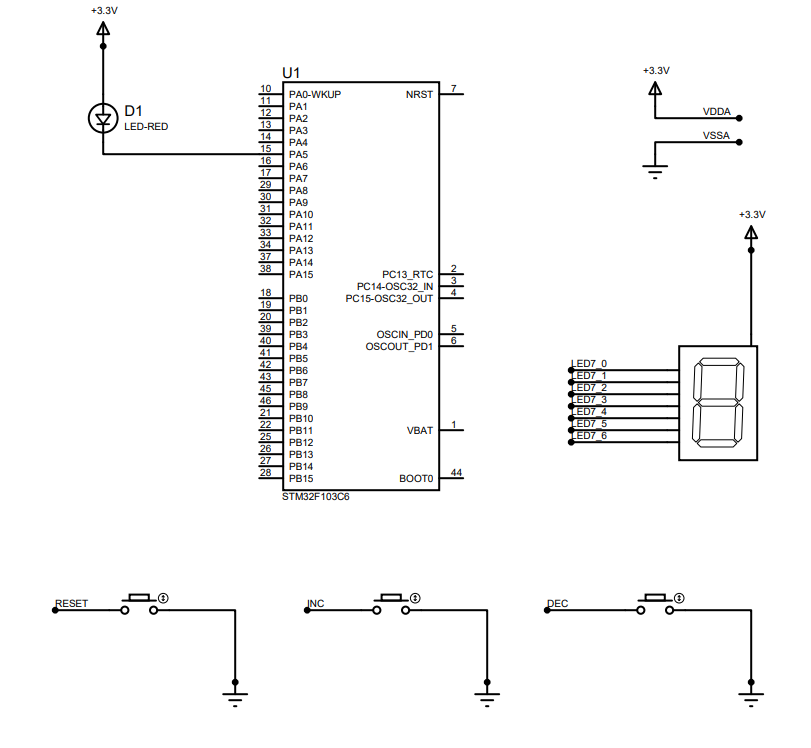
\includegraphics[width=5in]{source/picture/midterm/midtermschematic.PNG}
    \caption{\textit{Proteus schematic for count-down system}}
    \label{project_intro1}
\end{figure}

The main functions of the system are listed bellow:
\begin{itemize}
    \item LED7 segment is used to display a counter ranging from 0 to 9.
    \item The \textbf{RESET} button is used to reset the counter value to 0. Meanwhile, the \textbf{INC} and \textbf{DEC} buttons are used to increase and decrease the counter value, respectively. There are two events need to handle for these buttons, including the normal-press and long-press.
    \item The D1 LED is blinking every second, which is normally used to monitor the execution of the system.
\end{itemize}

Students are supposed to following the section bellow, to finalize the project and fill in reports for their implementations. Some important notes for your midterm are listed bellow:

\begin{itemize}
    \item The timer interrupt is 10ms. The value for counter is 9 (10 is also acceptable) when the pre-scaller is 7999.
    \item All the buttons must be DEBOUNCING by using a timer interrupt service routing. A timeout for long press event is 3 seconds.
    \item There is no HAL\_Delay() function in your source code. All the delay behavior must be based on a software timer.
    \item This report must be submitted with your answer.
    \item GitHub link for the source code and demo video link must be public access.
\end{itemize}

\section{Implement and Report}

\subsection{Proteus schematic - 1 point}
In this part, students propose the connection of the LED7 segment and 3 buttons to the STM32F103C6.\\

\textbf{Your report: } The schematic of your system is presented here. The screen can be captured and present in this part.\\


\subsection{State machine Step 1 - 2 points}
A state machine is required in this step to perform just only the normal-press (or a button push) behavior of three buttons:

\begin{itemize}
    \item Whenever the RESET is pressed, the counter value is 0.
    \item When INC is pressed, the counter is increased by 1. When counter is 9, it comes back to 0.
    \item When DEC is pressed, the counter is decreased by 1. When counter is 0, it rolls back to 9.
\end{itemize}

The value of the counter is displayed on the LED7 Segment.\\

\textbf{Your report: } Present your state machine in this part.\\

\textbf{Your report: } Present a main function, which is used to implement the state machine. This function should be invoked in main().

\begin{lstlisting}[caption=Implementation of the state machine]
void fsm_simple_buttons_run(){
    //TODO
}
\end{lstlisting}

\subsection{State machine Step 2 - 2 points}
In this part, long-press events for INC and DEC buttons are added to the project. For a button, this event is raised after 3 seconds keep pressing the button.\\

When a long-press event is detected, the value of counter keeps changing every 1 second until the button is released. For example, the current value of counter is 2 and the INC button is pressed. The value of counter immediately increased by 1,  or counter = 3. The INC button keeps pressing for 3 seconds, then the value of counter is 4. As long as the INC button is pressed, the value continues increasing \textbf{every 1 second}. This behavior is illustrated in the Figure bellow:

\begin{figure}[!htp]
    \centering
    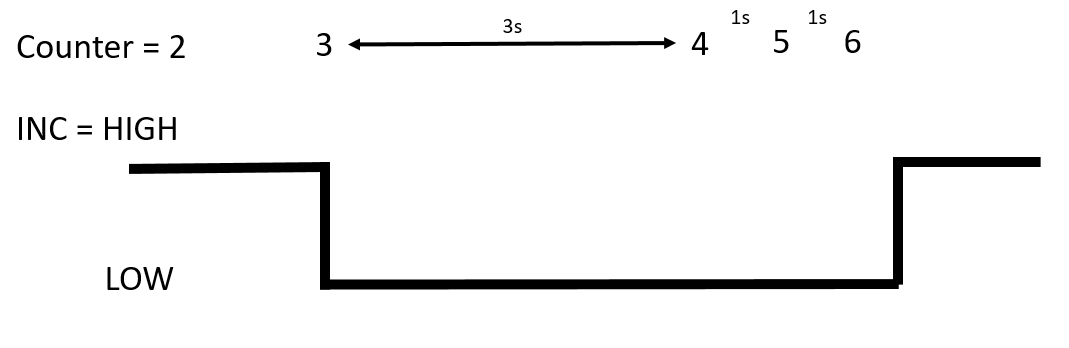
\includegraphics[width=5in]{source/picture/midterm/inclongpress.PNG}
    \caption{\textit{Long press behavior for INC button}}
    \label{longpress}
\end{figure}

The behaviors of the DEC button are reversed to the INC button. The value of counter is also roll back if it reaches 0 or 9.\\

\textbf{Your report: } Present your whole state machine when the long press events are added.\\

\textbf{Your report: } Present a main function, which is used to implement additional states. Minor changes in the previous source code are note required to present here.\\


\subsection{State machine Step 3 - 2 points}
Finally, where there is no button event after 10 seconds, the value of of counter is counted down and stopped at 0. If the INC or DEC are pressed again, the status of the system comes back to previous state, which is designed in Subsection 2 or 3.

\textbf{Your report: } Present your whole state machine for the 10s time-out event.\\

\textbf{Your report: } Present a main function, which is used to implement additional states. Minor changes in the previous source code are note required to present here.\\

\subsection{Led Blinky for Debugging - 1 point}

Finally, for many projects based on microcontroller, there is an LED keeps blinking every second. In this project, the LED connected to PA5 is used to perform this feature.\\

\textbf{Your report: } Present your solution and the source code for this feature. It can be very simple source code or a new state machine for this LED. If a state machine is used, please present it in the report.

\subsection{Github and Demo}

A link to your github presented the last commit of your project is provided in this section. This link contains all files in your STMCube project (configurations, header and source files)\\



\begin{center}
    \link{Your github link}
\end{center}


And a link for just one demo video is also needed to present here.


\begin{center}
    \link{Your video link}
\end{center}

  

\section{Extra exercise - Engineer mindset -1 point}
In this course, we encourage you to obtain an innovative mindset to solve daily problem. In this question, we would expect you to write a C program to solve the following problem. \\

Suffix with Unit\\

EXample:\\

1 suffixWithUnit(123) => 123\\

2 suffixWithUnit(1234) => 1.234 Kilo\\

3 suffixWithUnit(12345) => 12.345 Kilo\\

4 suffixWithUnit(1234567) => 1.234567 Mega\\

5 suffixWithUnit(12345678) => 12.345678 Mega\\


Prototype
\begin{lstlisting}
string suffixWithUnit(double number) {
}
\end{lstlisting}

How would you solve them? Please share your thinking to solve this problem and provide your answer.  


